

\section{Селективное лазерное спекание}
\subsection{Технология}
\subsection{Модель}

\section{Характеристиики полимеров для СЛС}

\subsection{Тепловые и механические параметры}
\subsection{"Тонкая" Структура}
\subsection{Полиэфиримиды ряда R-BAPB }
\subsection{Проблемы}

структура

Что следует из первичной структуры, термостойкость, особенности, пригодность для СЛС, перспективность

Данные по композитным добавкам

характеристики - все что измерили в ИВС

Что еще нужно выясеить

		
	\begin{figure}
	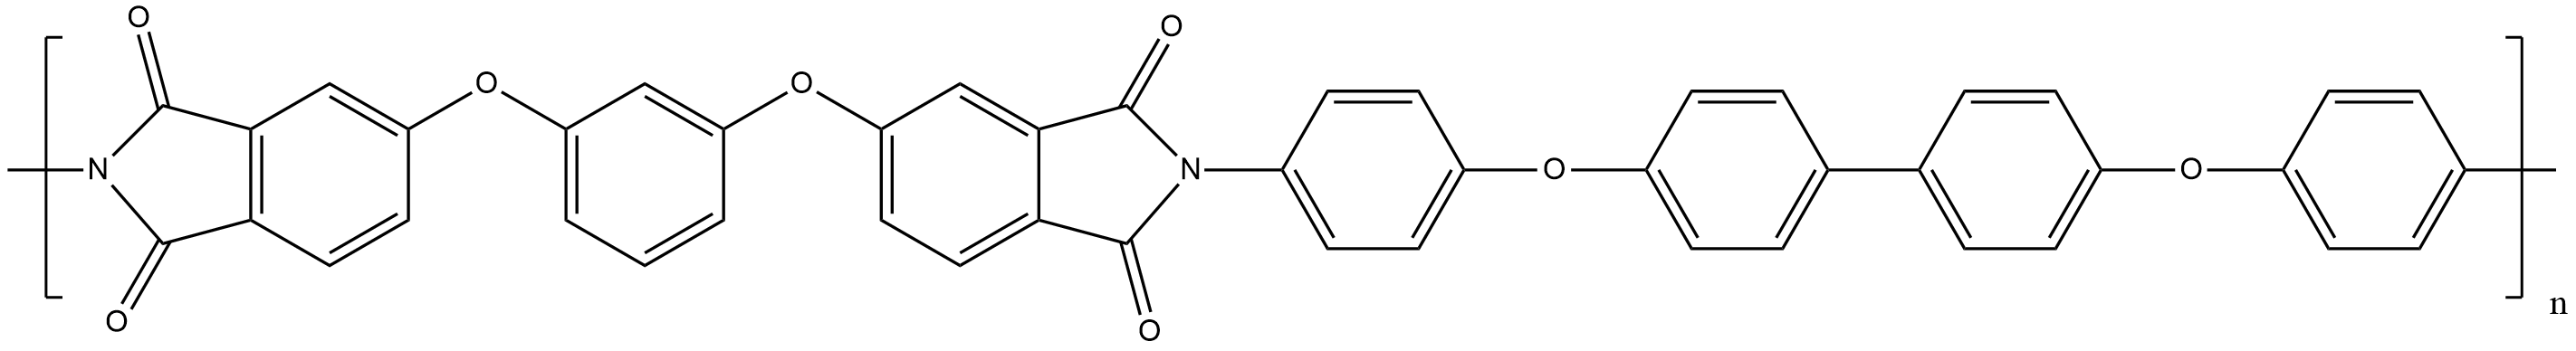
\includegraphics[width=\textwidth]{fig/formula.png}
	\end{figure}



\section{Кристаллическая структура полимеров}
\subsection{Кристаллиты}

	\begin{wrapfigure}{r}{0.5\textwidth} 
\vspace{-20pt}
  \begin{center}
    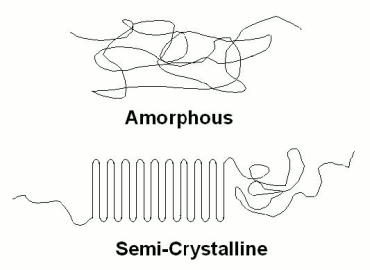
\includegraphics[width=0.4\textwidth]{fig/crystal-1.png}
    \caption{Как цепочки складываются в ламели}
    \label{fig:crystal-1}
  \end{center}
  \vspace{-20pt}
  \vspace{1pt}
\end{wrapfigure}



\begin{figure}
    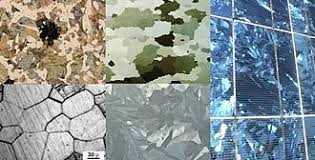
\includegraphics[width=\textwidth]{fig/crystallites.jpg}
    \caption{Типы кристаллитов}
    \label{fig:crystallites}
\end{figure}



\subsection{Частичная кристалличность}

	
	\begin{wrapfigure}{r}{0.5\textwidth} 
\vspace{-20pt}
  \begin{center}
    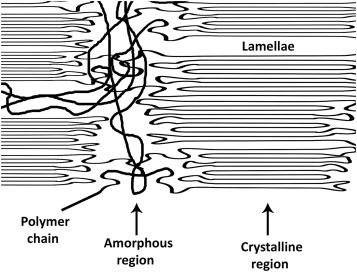
\includegraphics[width=0.4\textwidth]{fig/crystal-2.jpg}
    \caption{К определению кристалличности полимеров}
    \label{fig:crystal-2}
  \end{center}
  \vspace{-20pt}
  \vspace{1pt}
\end{wrapfigure}	

\subsection{Влияние на макроскопические параметры}

\section{Исследование кристаллической структуры}
\subsection{ЯМР}
\subsection{Еще что-то}
\subsection{Сравнение и обоснование}
тут методы, обоснование

\section{Исследование структуры с помощью дифракции рентгеновского рассеяния}

\subsection{Синхротронное излучение}
когерентные источники, йоу!
\subsection{Упругое рассеяние}
\subsection{2D-снимки, порошковая дифракция}
\subsection{Неупругое рассеяние,гало}
эффекты от аморфной части



	